\section{Design of the LNA}

In this section, we present the design of the LNA architecture shown in Figure \ref{fig:schem-lna}. The design process involves biasing conditions and ensuring the desired specifications are met.

The LNA architecture combines a common-gate (CG) stage in parallel with a common-source (CS) stage at the input. In this configuration, the overall input impedance is the parallel combination of the CS and CG input impedances: $Z_\text{in} = Z_\text{CS} // Z_\text{CG}$. Ideally, the common-source path presents an effectively infinite input impedance, so $Z_\text{CS} \approx +\infty$. As a result, the input impedance is dominated by the common-gate device, which can be designed to be around \SI{50}{\ohm}.

\label{sec:inpCap}
However, at high frequencies, the parasitic input capacitances of the transistors become significant. In practice, the “infinite” input impedance of the CS path is shunted by the devices' capacitances. Although smaller nodes have smaller input capacitances, this effect is exacerbated, because they are intended to work in higher frequencies.

The design process followed a workflow that began with theoretical calculations using standard MOSFET equations to estimate $g_m$, $I_D$, and transistor dimensions. These initial values were generated via a Python script. The preliminary design was then simulated using LTSpice, where an operating point (\texttt{.op}) analysis provided accurate values for parameters like $g_{ds}$ and $g_{mb}$. Given that $r_{ds}$ is difficult to estimate analytically, it was refined post-simulation, and the design was recalculated using the updated values. Final adjustments were made through iterative fine-tuning according to the device equations, ensuring that the LNA met the specified gain and impedance requirements.

\label{sec:assumptions}
In the initial design phase, it was assumed that $g_{ds} \ll g_m$ and that the body-effect transconductance could be approximated as $g_{mb} \approx 0.2\,g_m$. A fixed overdrive voltage of $V_{DSsat} = \SI{100}{\milli\volt}$ was used to ensure that all transistors operated in the correct zone. Device sizing and biasing were based on standard saturation-region MOSFET Equations \ref{eq:gm_eq}, \ref{eq:ID_eq} and $g_{ds} \propto \frac{L}{I_D}$\cite{AnalogCircDesign}. These expressions guided the theoretical design and were iteratively validated and adjusted during simulation.

\begin{equation}
    g_m =\sqrt{2K_{n,p}\frac{W}{L}I_D}= \frac{2I_D}{V_{DSsat}}
    \text{\cite{AnalogCircDesign}}
    \label{eq:gm_eq}
\end{equation}

\begin{equation}
    I_D=\frac{K_n}{2}\cdot\frac{W}{L}V_{DSsat}^2
    \text{\cite{AnalogCircDesign}}
    \label{eq:ID_eq}
\end{equation}

\subsection{Common Gate Stage Design}

The schematic presented in Figure \ref{fig:CG_SmallSignal} corresponds to the small signal model of the common-gate stage. From it, the relevant expressions for the design of this stage were derived. 

\begin{figure}[H]
    \centering
    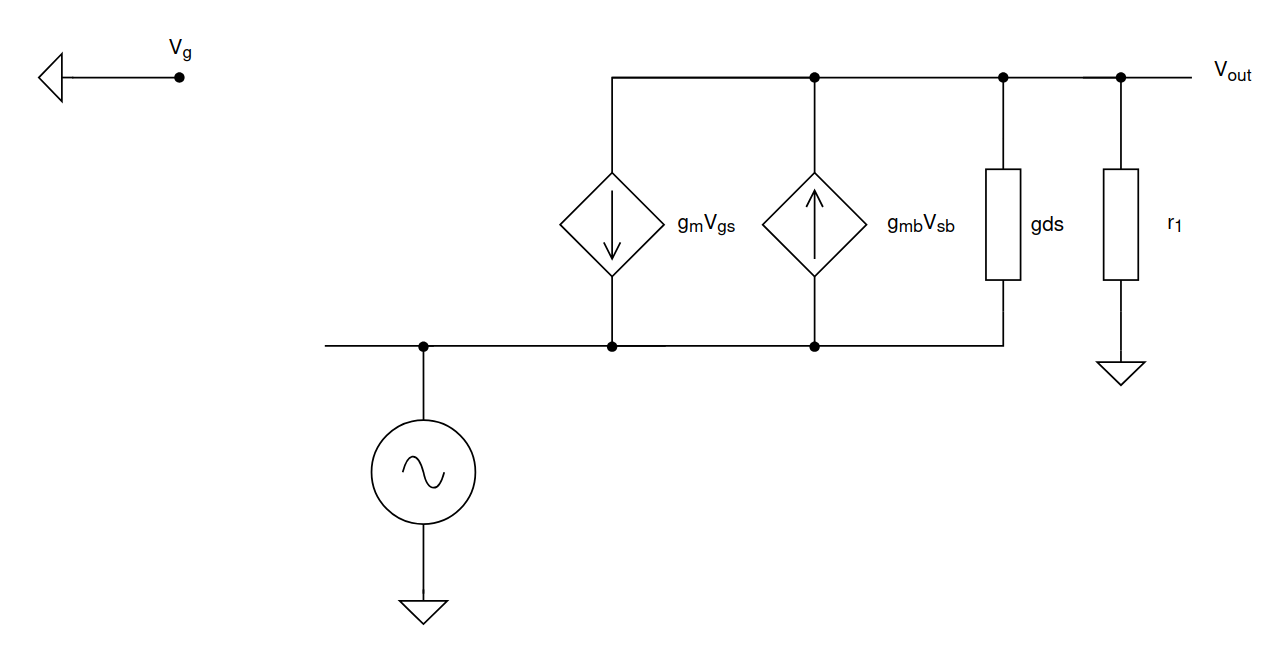
\includegraphics[width=1\textwidth]{Images/CG_SmallSignal.png}
    \caption{Common Gate Small Signal Schematic.}
    \label{fig:CG_SmallSignal}
\end{figure}

In order to meet, the specifications, Table \ref{tab:specifications}, the necessary Equations are Gain and Input impedance, Equations \ref{eq:CG_Gain} and \ref{eq:CG_Zin}, respectively.

\begin{equation}
    A_v = \frac{v_o}{v_i}=\frac{g_m+g_{mb}+g_{ds}}{g_{ds}+1/r_1}
    \label{eq:CG_Gain}
\end{equation}

\begin{equation}
    Z_{in} = \frac{V_i}{I_i}=\frac{1}{- \frac{g_{ds} \left(g_{ds} + \frac{1}{r_{1}}\right)}{g_{ds} + g_{m} + g_{mb}} + g_{ds} + g_{m} + g_{mb}}\approx\frac{1}{g_m+g_{mb}}
    \label{eq:CG_Zin}
\end{equation}

\subsubsection{Circuit sizing}

Using the approximation presented in section \ref{sec:assumptions}, where $g_{mb} \approx 0.2\,g_m$, and Equation \ref{eq:CG_Zin} for input impedance, it is possible to determine the required $g_m$ to meet the input matching specification. For $Z_{in} = \SI{50}{\ohm}$, this gives $g_m \approx \SI{16.667}{\milli\siemens}$.

With this $g_m$ and the initial value of $V_{DSsat} = \SI{100}{\milli\volt}$, the drain current $I_D$ can be calculated using Equation \ref{eq:gm_eq}.

Once $I_D$ is known, the value of the transistor aspect ratio $W/L$ can be obtained using Equation \ref{eq:ID_eq}.

To meet the gain specification, Equation \ref{eq:CSGain} shows that the voltage gain depends on the value of $r_1$, since $g_m$ and $g_{mb}$ are already fixed from the input matching requirement. Therefore, $r_1$ is chosen to achieve the desired gain.

As $I_D$ is imposed by a current source, the value of $V_{DSsat}$ is maintained fixed. Thus, the bias voltage $V_{bias}$ must be set such that $V_s > 0$, to ensure proper transistor operation, but also such that $V_s < V_d$.

This sets a constraint on $V_{bias}$, which must guarantee the correct operation region for the common-gate transistor.
 
\subsection{Common Source Stage Design}


\begin{figure}[H]
    \centering
    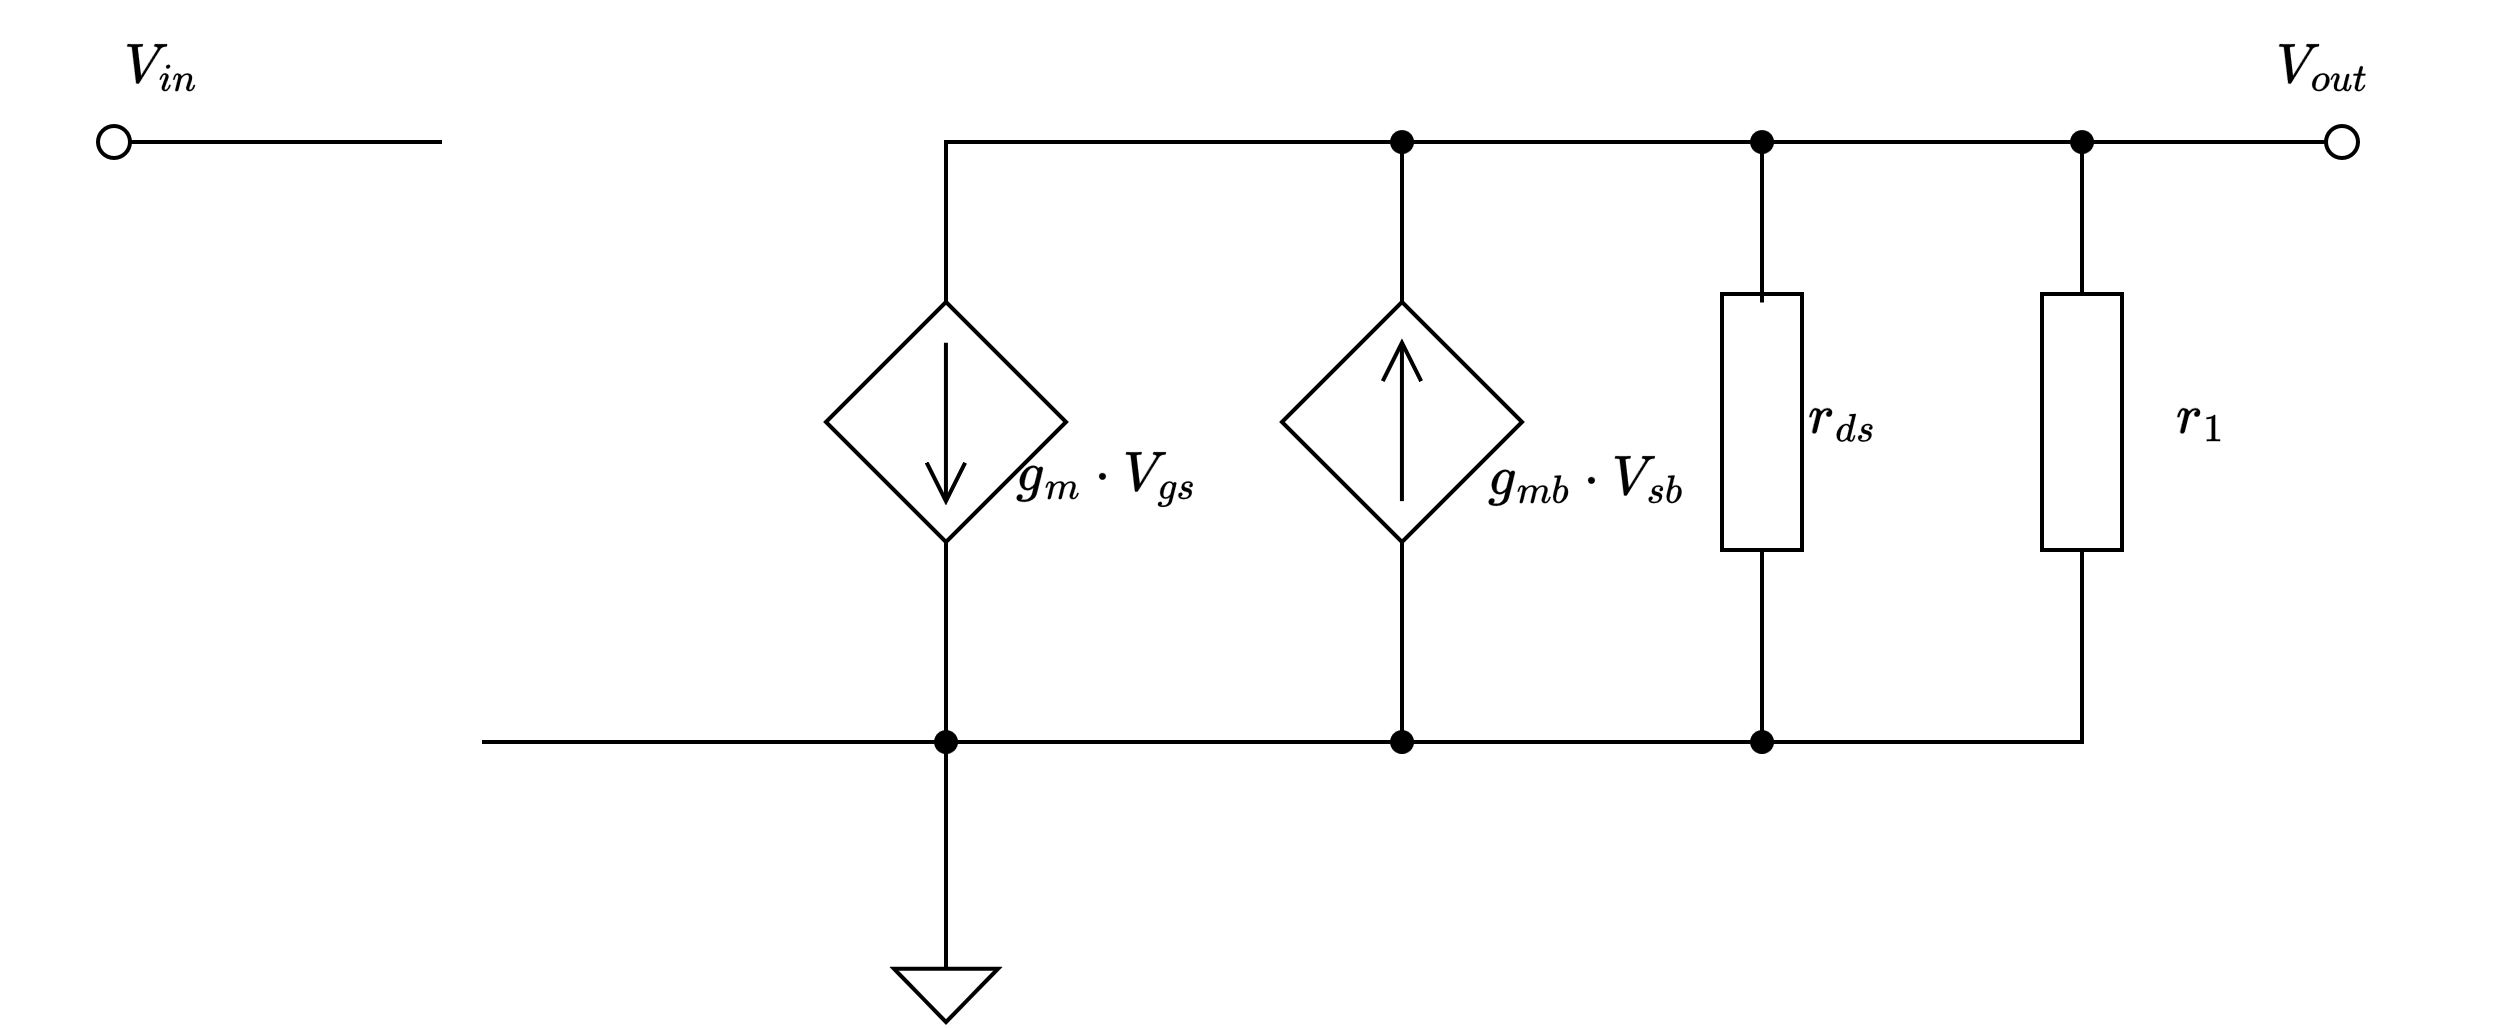
\includegraphics[width=1\textwidth]{Images/CS_SmallSig.png}
    \caption{Common Source Small Signal Schematic.}
    \label{fig:CS_SmallSignal}
\end{figure}

Figure \ref{fig:CS_SmallSignal} shows the small signal equivalent circuit for the common-source stage. From this schematic, the expression for voltage gain can be determined, Equation \ref{eq:CS_Gain}. As already explained in section \ref{sec:assumptions} the common-source input impedance is not relevant.

\begin{equation}
    A_v = -g_m \left( r_{ds} // R_L \right)
    \label{eq:CS_Gain}
\end{equation}

\subsubsection{Circuit Sizing}

For the common-source stage, the input impedance is not a design concern, although the input capacitances will have a significant effect on circuit performance, as discussed in Section \ref{sec:inpCap}.

Certain parameters are fixed, such as $V_{DSsat}$, to ensure that the device operates in the saturation region. The transconductance $g_m$ will take on two values during the design process: initially, it will match the value used in the common-gate stage, and in a second phase, it will be set to three times that value.

With these fixed values, $W/L$ can be obtained using Equation \ref{eq:gm_eq} and rewritten as Equation \ref{eq:wl2}.

\begin{equation}
    \begin{split}
        g_{m_1} &= n\cdot g_{m_2} = K_{n}\frac{W}{L}V_{DSsat} \text{\cite{AnalogCircDesign}} \Leftrightarrow \\
        \Leftrightarrow \frac{W}{L} &= \frac{g_{m2}}{K_n \cdot V_{DSsat}^2}
    \end{split}
    \label{eq:wl2}
\end{equation}

The resistor $r_2$ is sized based on the desired voltage gain using Equation \ref{eq:r2}.

\begin{equation}
    r_2 = - \frac{A_v \cdot r_{ds}}{A_v - g_m \cdot r_{ds}}
    \label{eq:r2}
\end{equation}

In this stage, the calculation of $V_{bias}$ is straightforward, since $V_{GS} = V_{bias}$ and $V_{DSsat} = V_{GS} - V_{th}$. This leads to the Equation \ref{eq:V_bias_CS}.

\begin{equation}
    V_{bias} = V_{GS} = V_{DSsat} + V_{th}
    \label{eq:V_bias_CS}
\end{equation}


\subsection{Buffer Stage Design}

\begin{figure}[H]
    \centering
    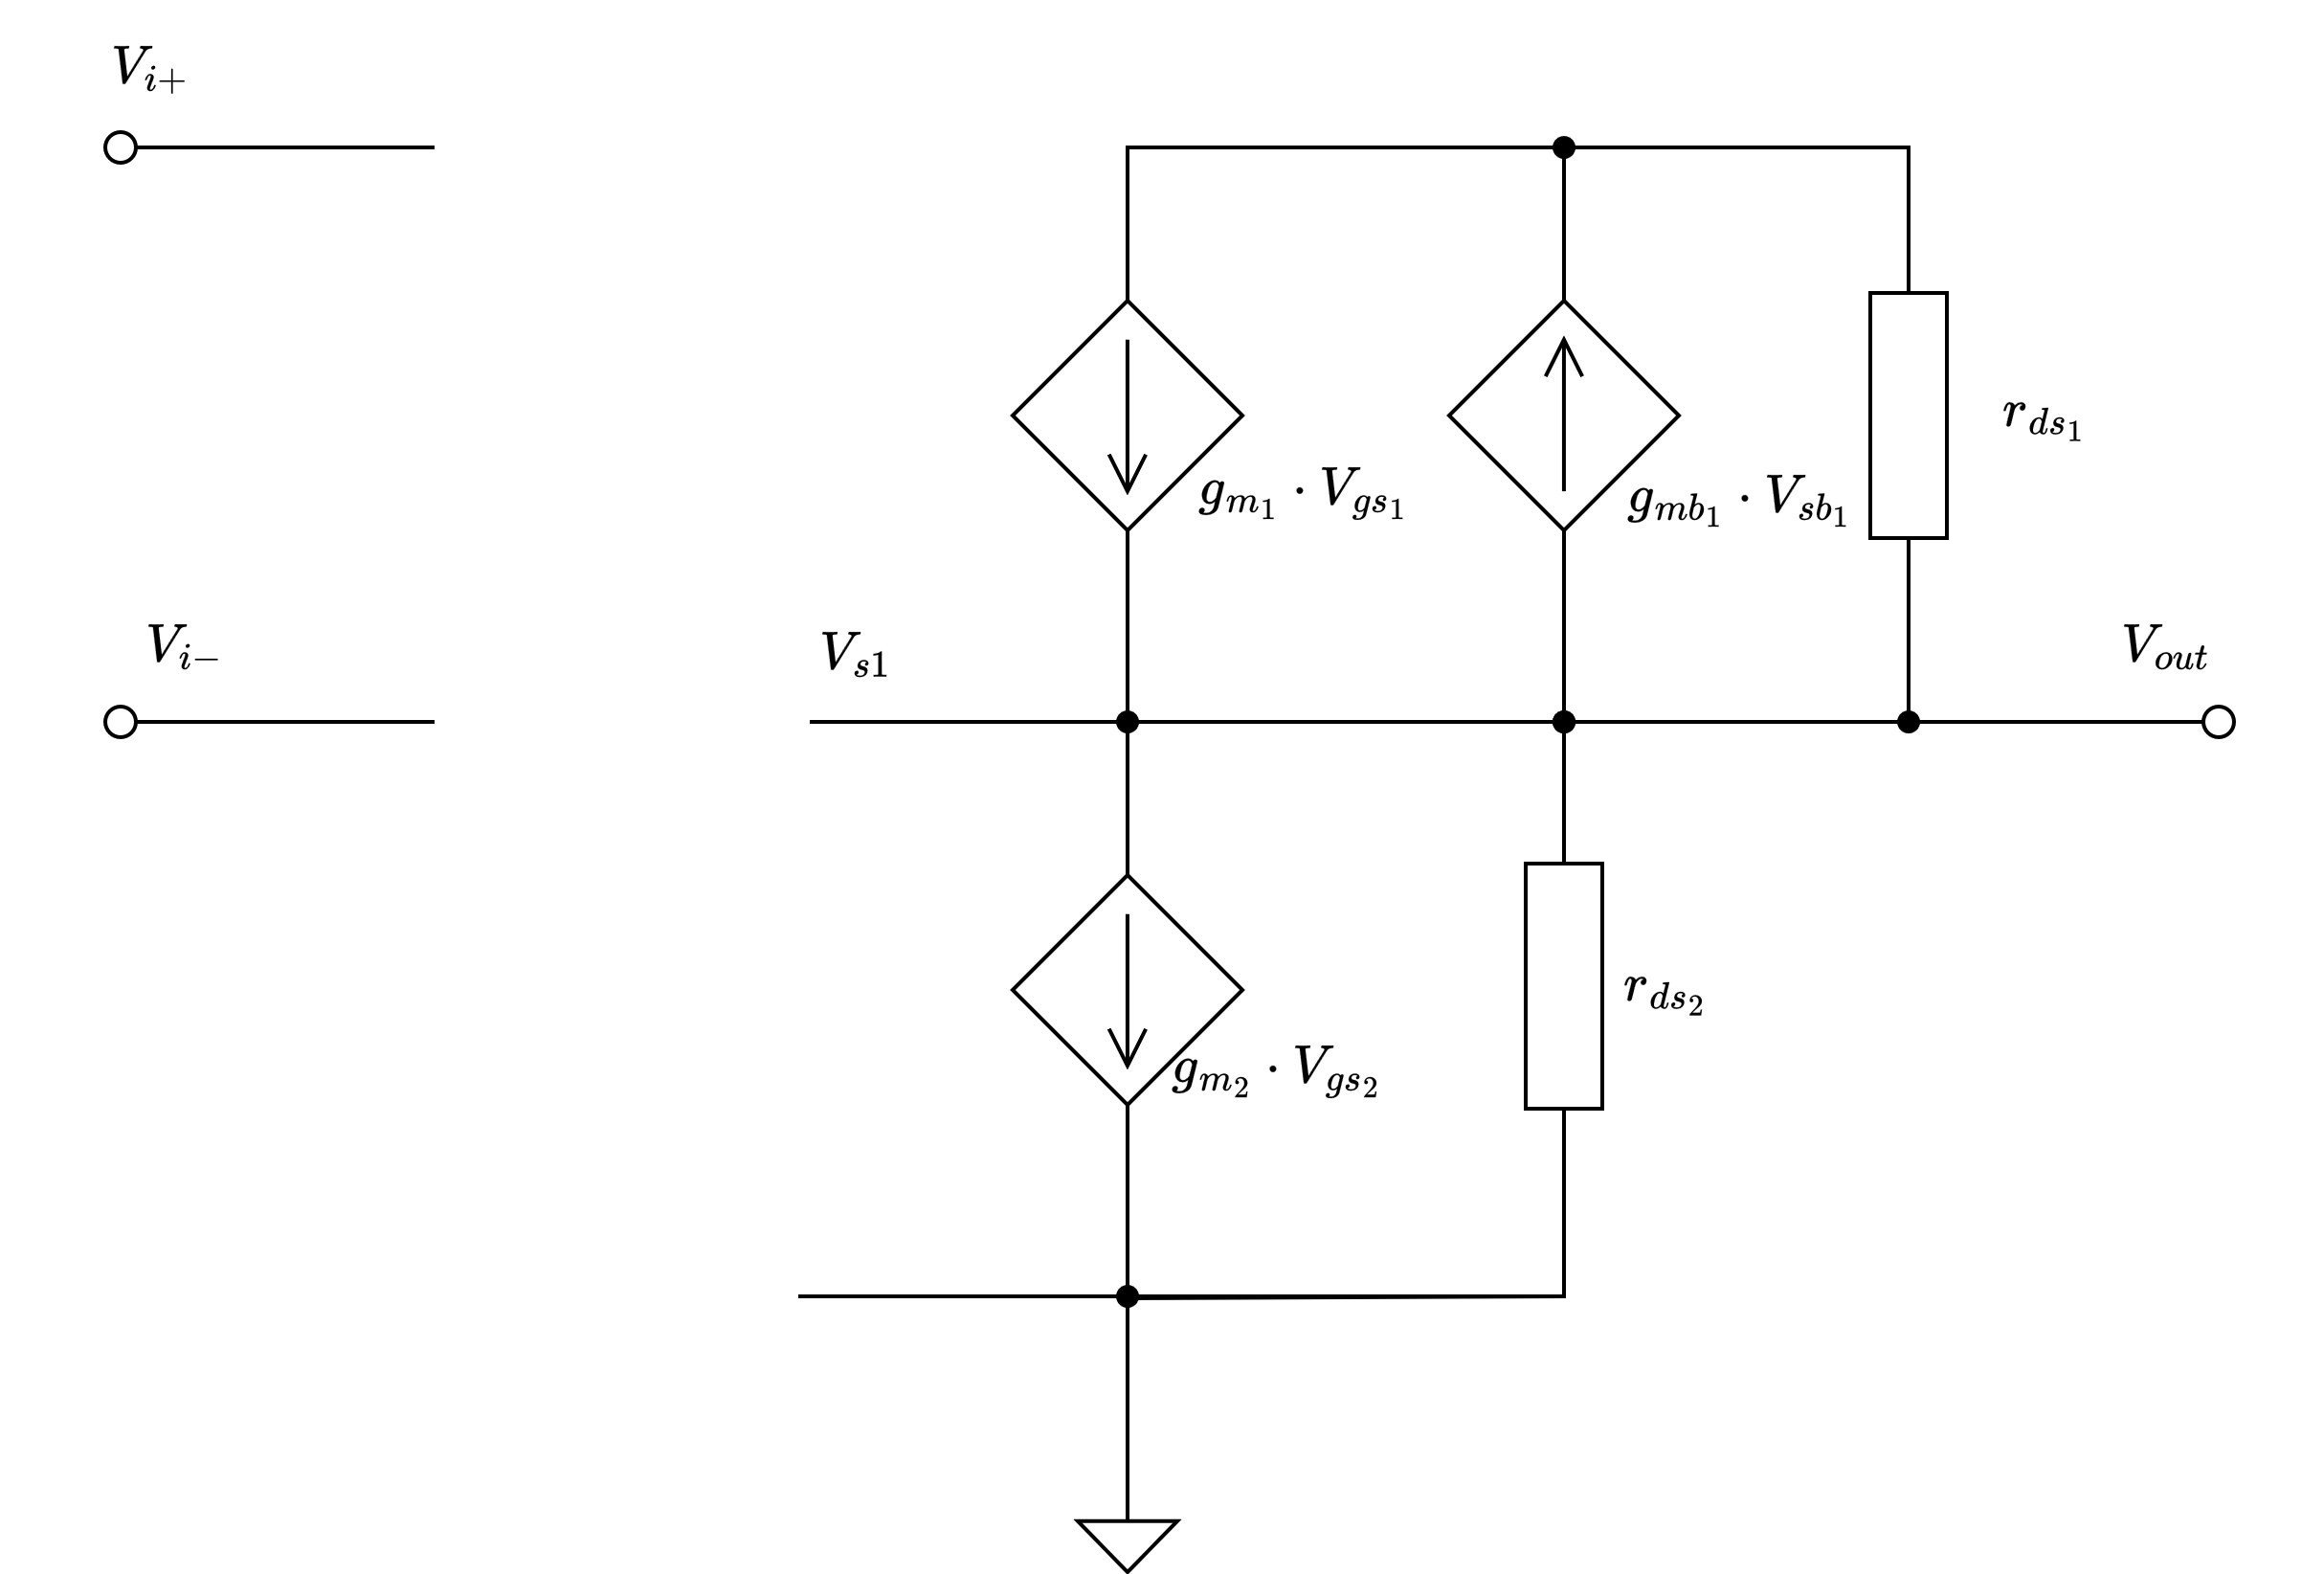
\includegraphics[width=0.8\textwidth]{Images/BufferSmallSignal.png}
    \caption{Buffer Small Signal Schematic.}
    \label{fig:Buff_SmallSignal}
\end{figure}

Figure \ref{fig:Buff_SmallSignal} shows the small signal schematic for the Voltage-combiner buffer stage. This block is responsible for providing low output impedance, making the output single-ended and isolating the LNA core from the load, ensuring that the previous stages are not affected by the external circuitry.

The gain of the buffer is given by Equation \ref{eq:buff_Gain}.
\begin{equation}
    A_v =  \frac{g_{m2}+ g_{m1}}{g_{ds1}+g_{ds2}+g_{mb1}+g_{m1}} \approx 1 + \frac{g_{m2} }{g_{m1}}
    \label{eq:buff_Gain}
\end{equation}

Where the approximation holds assuming that $g_{m1}$ is much larger than $g_{ds}$ and $g_{mb1}$.

The output impedance is approximated by Equation \ref{eq:buff_zout}.
\begin{equation}
    Z_{out} = \left(\frac{1}{g_{m1}}\right) // r_{ds_2} \approx \frac{1}{g_{m1}}
    \label{eq:buff_zout}
\end{equation}

Maintaining the assumption that $g_{m1} \gg g_{ds}$, to ensure the specification is met, Table \ref{tab:specifications}, it is necessary that $g_{m1} \approx \SI{20}{\milli\siemens}$

From the Equation \ref{eq:buff_Gain}, it is clear that for the buffer to operate close to unity gain and present the desired output impedance, the transistors should have similar characteristics, and $g_{m1} \approx g_{m2}$. 

The biasing voltages were calculated based on the target DC operating point of the buffer. For the transistor $M_4$, Figure \ref{fig:schem-buffer}, the gate voltage was defined as:
\[
    V_{biasn} = V_{GS} = V_{tn} + V_{DSsat},
\]
For the $M_3$ transistor, Figure \ref{fig:schem-buffer}, it was assumed that the DC output voltage should be centered at $V_{DD}/2$, so the gate voltage was chosen as:
\[
    V_{biasp} = \frac{V_{DD}}{2} + V_{GS},
\]
with $V_{GS}$ equal to the transistor $M_4$. This guarantees symmetrical swing and proper headroom for the output stage.

\subsection{Initial Values}

Using the python script developed with the these equations, Appendix \ref{appendix:python_script}, the initial values were calculated, Tables \ref{tab:initial-vals-cg} and \ref{tab:initial-vals-cs}. 

\begin{table}[H]
    \centering
    \footnotesize
    \caption{Initial Values for the CG stage}
    \begin{tabularx}{\textwidth}{>{\centering\arraybackslash}X 
                                >{\centering\arraybackslash}X 
                                >{\centering\arraybackslash}X 
                                >{\centering\arraybackslash}X 
                                >{\centering\arraybackslash}X 
                                >{\centering\arraybackslash}X
                                >{\centering\arraybackslash}X}
        \toprule
        Node & $g_m$ ratio & W & L & $g_m$ (mS) & R ($\si{\ohm}$) & $V_{bias}$ (mV)  \\
        \midrule

        \multirow{1}{*}{350nm}
        &  1:1 & $\SI{291}{\micro\meter}$ & $\SI{350}{\nano\meter}$  & $15.9$ & $280$ & $1500$  \\

        \midrule
        \multirow{1}{*}{65nm}
        & 1:1 & xxx  & xxx & xxx & xxx  & xxx \\
        
        \midrule
        \multirow{1}{*}{45nm}
        &  1:1 & \SI{642}{\micro\meter}  & \SI{135}{\nano\meter} & 17.3 & 286 & 352 \\


        \bottomrule
    \end{tabularx}
    \label{tab:initial-vals-cg}
\end{table}

\begin{table}[H]
    \centering
    \footnotesize
    \caption{Initial values for the CS stage}
    \begin{tabularx}{\textwidth}
        {@{}%  ⟵ trim left padding
         >{\centering\arraybackslash}X
         *{6}{>{\centering\arraybackslash}X}@{}} % ⟵ trim right padding
        \toprule
        Node & Config & W (\si{\micro\meter}) & L (\si{\nano\meter})
             & $g_m$ (mS) & R (\si{\ohm}) & $V_\text{bias}$ (mV) \\
        \midrule
        \multirow{2}{*}{\SI{350}{\nano\meter}}
            & 1:1 & \SI{291}{\micro\meter} & \SI{350}{\nano\meter} & 17.0 & 334 & 670 \\
            & 1:n & \SI{875}{\micro\meter} & \SI{350}{\nano\meter} & 51.8 &  103 & 700 \\
        \midrule
        \multirow{2}{*}{\SI{65}{\nano\meter}}
            & 1:1 & --- & --- & --- & --- & --- \\
            & 1:n & --- & --- & --- & --- & --- \\
        \midrule
        \multirow{2}{*}{\SI{45}{\nano\meter}}
            & 1:1 & \SI{450}{\micro\meter}  & \SI{135}{\nano\meter}  & 17.8 & 760 & 385 \\
            & 1:n & \SI{1350}{\micro\meter} & \SI{135}{\nano\meter} & 59.5 & 125 & 455 \\
        \bottomrule
    \end{tabularx}
    \label{tab:initial-vals-cs}
\end{table}

